\documentclass[12pt,letterpaper]{article}
\usepackage[margin=.84in,top=.80in,bottom=.79in,headheight=15pt,headsep=18pt]{geometry}
\usepackage{amsmath,amssymb,amsthm,booktabs,array,xcolor,tikz,fancyhdr,hyperref}
\usetikzlibrary{arrows.meta,positioning,calc}
\definecolor{ink}{HTML}{183448}
\definecolor{accent}{HTML}{16634E}
\definecolor{rust}{HTML}{963E31}
\definecolor{blueink}{HTML}{215D91}
\definecolor{soft}{HTML}{EAF3EE}
\definecolor{muted}{HTML}{48616B}
\hypersetup{colorlinks=true,linkcolor=accent,citecolor=accent,urlcolor=blueink,
pdftitle={Two blue clues in cubic bipartite edge coloring},pdfauthor={Research note prepared for Dominic Dabish}}
\pagestyle{fancy}\fancyhf{}
\fancyhead[L]{\sffamily\footnotesize\color{accent} GRAPH COLORING}
\fancyhead[R]{\sffamily\footnotesize\color{muted} MATCHINGS AND RECONFIGURATION}
\fancyfoot[L]{\sffamily\footnotesize\color{muted} Research note for Dominic Dabish \enspace / \enspace 21 November 2026}
\fancyfoot[R]{\sffamily\footnotesize\color{muted}\thepage}
\renewcommand{\headrulewidth}{.35pt}
\setlength{\parindent}{0pt}\setlength{\parskip}{5pt}
\setlength{\abovedisplayskip}{7pt}\setlength{\belowdisplayskip}{7pt}
\setlength{\emergencystretch}{1.2em}
\newcommand{\hd}[1]{\par\medskip{\large\bfseries\color{accent}#1}\par\nobreak}
\newcommand{\sh}[1]{\par\smallskip{\bfseries\color{ink}#1}\quad}
\newcommand{\Sec}[1]{\section{\color{ink}#1}}
\newcommand{\sat}{\mathrm{SAT}}
\newcommand{\cnt}{\mathop{\#\mathrm{SAT}}}
\newcommand{\cyc}{\operatorname{cyc}}
\newcommand{\note}[1]{\par\smallskip\noindent\colorbox{soft}{\parbox{\dimexpr\linewidth-2\fboxsep\relax}{\vspace{4pt}#1\vspace{4pt}}}\par\smallskip}
\newcommand{\rs}{\textcolor{rust}{\textsf{red}}}
\newcommand{\bs}{\textcolor{blueink}{\textsf{blue}}}
\newcommand{\rref}[2]{\href{#1}{#2}}
\begin{document}
\phantomsection\pdfbookmark[1]{Main result}{main}
{\sffamily\small\color{muted} COMPUTATIONAL COMPLEXITY \hfill WORKING MANUSCRIPT}\\[6pt]
{\fontsize{27}{31}\selectfont\bfseries\color{ink} Two blue clues in cubic\\[1pt] bipartite edge coloring\par}
\vspace{3pt}
{\large\color{muted} A linear-size reduction preserving the SAT solution graph\par}
\vspace{6pt}
Does a partially colored graph admit a proper coloring of its edges with red, blue and green? We study connected simple bipartite graphs with degree three at every vertex. The palette always has three colors. Only red and blue occur among the clues.

\note{\textbf{Threshold.} With arbitrarily many red clues and at most one blue clue, extension is decidable in polynomial time. With exactly two blue clues it is NP-complete, even when \emph{all} prescribed edges form a matching and the red clues cover exactly half the vertices.}

\hd{An assignment-preserving theorem}
Let \(F\) be a CNF formula with \(n\ge1\) occurring variables, \(m\ge1\) nonempty clauses and \(L\) literal occurrences. In polynomial time one can construct a graph with \(N=256L+4n+16\) vertices. Its red perfect matchings containing the red clues are indexed bijectively by \(x\in\{0,1\}^n\). Every one avoids both blue edges. Removing a red matching leaves even cycles. Let \(B(M)\) count the cycles on which the blue clues cannot be satisfied by alternating blue and green. Then
\[
                              B(M_x)=1-F(x).
\]
Here true is \(1\). Each satisfied assignment lifts to exactly the same explicit power of two full colorings. Two red matchings differ by one alternating-cycle flip exactly when their assignments differ in one bit.

\hd{What the theorem decides}
The reduction transfers SAT, model counting and solution-path reachability to one family of graphs. It also yields a tight conditional base \(2\) for enumeration by the number of independent red-matching cycles. With only the red clues imposed, a full extension can be sampled exactly in linear time on the constructed family. The probability that both probe edges are blue equals \(\cnt(F)/(4\cdot2^n)\).

\sh{Relation to previous work.}
Two-color precoloring hardness on cubic bipartite graphs was explicitly recorded by Fiala, Kratochv\'il and P\'or in 2005 \cite{fkp}. Kratochv\'il and Seb\H{o} had already obtained a multiplicity threshold for vertex coloring on the broader class of perfect graphs \cite{ks}. This note gives an explicit two-blue-edge construction in the cubic bipartite class. Priority and validity have not undergone external peer review. P versus NP remains open \cite{clay}.

\newpage
\Sec{A reversible test for CNF satisfiability}
The first construction produces a permutation \(P_x\) of a set of lanes. Two designated lanes lie in different cycles of \(P_x\) exactly when \(x\) satisfies \(F\). Conditional instructions are controlled by individual Boolean variables. Each instruction acts on a constant number of lanes, apart from one fixed permutation.

\sh{Lanes.}
Let the clause lengths be \(\ell_1,\ldots,\ell_m\) and \(k=\max_i\ell_i\). Give a central group the layers \(0,\ldots,k\) and give clause group \(i\) its own layers \(0,\ldots,\ell_i\). Duplicate each lane into rails \(b=0,1\). The number of lanes is
\[
                  W=2\bigl(k+1+L+m\bigr).
\]
Write a lane as \((g,r,b)\) for group, layer and rail. The two marked lanes are \(h_b=(0,0,b)\). Layer zero will carry the result.

\sh{One clause.}
For clause \(i\), read its literals in order. If literal \(j\) is true, interchange layers \(0\) and \(j\) in \emph{both} groups \(0,i\) and on \emph{both} rails. This acts by four disjoint transpositions. Write the sequence as \(U_i\). Next interchange the two groups at layer zero on both rails regardless of the input. Finally undo \(U_i\).
The net result interchanges the two groups at exactly one layer on both rails. This is layer zero if every literal is false. Otherwise it is the index of the last true literal. To see this, apply \(U_i^{-1}\) to layer zero. The first executed true swap takes it to that index and the remaining swaps leave the index alone.

\sh{All clauses.}
Concatenate these clause permutations in order to form \(S_x\). Starting on \(h_b\), a satisfied clause leaves the central lane on layer zero unchanged. The first falsified clause sends it to that clause's private layer-zero lane. Later clauses use different private groups, so it stays there. The rail is preserved in either event.

\sh{Compare two copies of the result.}
Let \(T\) swap \((i,0,0)\) with \((i,0,1)\) for each \(1\le i\le m\). Let it fix every other lane. Execute \(S_x,T,S_x^{-1}\), giving \(P_x=S_x^{-1}TS_x\). On a satisfying assignment, \(P_x\) fixes \(h_0,h_1\) separately. On any other assignment it transposes them. Moreover
\[
                           \cyc(P_x)=\cyc(T)=W-m
\]
for every assignment. A failed clause changes the locations of cycles while preserving their total number. This identity will make the lift multiplicity independent of the satisfying assignment.

\begin{center}
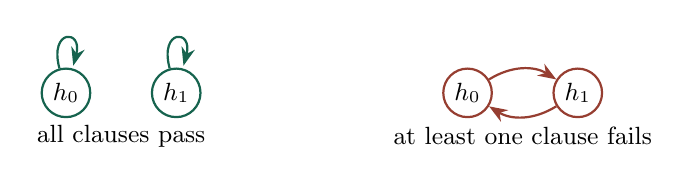
\begin{tikzpicture}[>=Stealth, every node/.style={font=\small}, thick]
\begin{scope}
\node[circle,draw=accent,inner sep=2pt] (a) at (0,0) {$h_0$};
\node[circle,draw=accent,inner sep=2pt] (b) at (1.4,0) {$h_1$};
\path[->,accent] (a) edge[loop above] (a) (b) edge[loop above] (b);
\node at (.7,-.55) {all clauses pass};
\end{scope}
\begin{scope}[xshift=5.1cm]
\node[circle,draw=rust,inner sep=2pt] (c) at (0,0) {$h_0$};
\node[circle,draw=rust,inner sep=2pt] (d) at (1.4,0) {$h_1$};
\draw[->,rust] (c) to[bend left=32] (d);
\draw[->,rust] (d) to[bend left=32] (c);
\node at (.7,-.55) {at least one clause fails};
\end{scope}
\end{tikzpicture}
\end{center}

\sh{Size.}
Each literal occurs four times as a conditional instruction in the entire sequence. Each occurrence handles eight lanes. A negative literal is implemented by its fixed permutation followed by the same involution controlled on the positive variable. Fixed permutations are wired directly. Lanes untouched between consecutive uses are joined by one wire. Every lane is touched, since each private layer appears in its clause and the longest clause uses every central layer.

\newpage
\Sec{One cycle controls every use of a variable}
Think of a port as a position with an input vertex on the left and an output vertex on the right. Every input and output will eventually have one external wire. The graph will force those wires to be nonred. Inside a variable's cycle, a red perfect matching can take either alternating half. The other half pairs inputs to outputs and routes their binary wire values.

\sh{External ports.}
Suppose variable \(v\) occurs \(d\) times in the formula. Collect its \(q=32d\) touched lane positions from the program. We need to route these external ports identically when \(x_v=0\) and by a permutation \(\tau\) when \(x_v=1\). Here \(\tau\) is the product of all disjoint instruction swaps on their \emph{distinct occurrence ports}. The same logical lane at different times has distinct ports. Order the endpoints of each two consecutive swaps \((a\,b),(c\,d')\) as \(a,c,b,d'\). In each block of four, \(\tau\) now interchanges the first with the third and the second with the fourth.

\sh{The cycle.}
Place \(A_i,B_i\) in that order for every \(i\) modulo \(q\), giving \(2q\) cyclic positions. The \(A_i\) are external. At position \(j\) put \(L_j,R_j\). Draw \(L_jR_j\) and \(L_jR_{j+1}\), with indices modulo \(2q\). Their union is one even cycle. Its two complementary routing choices send every input straight or every input forward by one position. Join the output of internal position \(B_i\) by a wire to the input of \(B_{\pi(i)}\), where \(\pi(i)=\tau(i)-1\bmod q\).
\[
  A_i \xrightarrow{\text{shift}} B_i\text{ out}
      \xrightarrow{\text{wire}} B_{\pi(i)}\text{ in}
      \xrightarrow{\text{shift}} A_{\pi(i)+1}=A_{\tau(i)}\text{ out}.
\]
In straight mode each external port is fixed, and the internal positions form the cycles of \(\pi\). In shifted mode all internal positions occur on external routes and none forms a separate cycle. In a block numbered \(0,1,2,3\) locally, \(\pi\) traverses \(3,0,1,2\) and then the last position of the previous block. Hence \(\pi\) has exactly one cycle.

\sh{One internal cycle in both modes.}
Introduce a balancing position \(z\). Replace \(L_0R_0\) by the three-edge path \(L_0,R_z,L_z,R_0\), and join the output of \(z\) by a wire to its input. In straight mode the route from \(L_0\) to \(R_0\) detours through the \(z\)-wire. In shifted mode \(L_zR_z\) and that wire form one internal cycle. The external maps are unchanged. Both modes now contribute one internal cycle.

\begin{center}
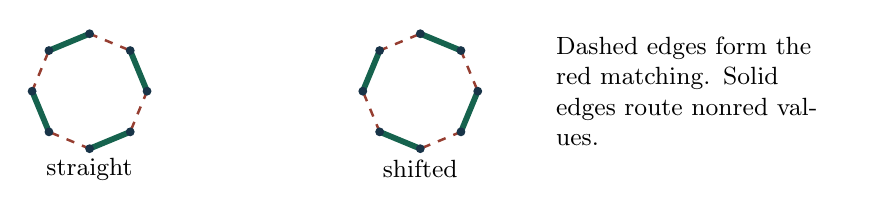
\begin{tikzpicture}[every node/.style={font=\small}]
\foreach \off/\state/\labelname in {0/0/straight,4.2/1/shifted}{
\begin{scope}[xshift=\off cm]
\foreach \i in {0,...,7}{
\pgfmathtruncatemacro{\j}{mod(\i+1,8)}
\pgfmathtruncatemacro{\p}{mod(\i+\state,2)}
\ifnum\p=0\draw[rust,dashed,line width=.9pt] ({90-45*\i}:.73)--({90-45*\j}:.73);
\else\draw[accent,line width=2.1pt] ({90-45*\i}:.73)--({90-45*\j}:.73);\fi}
\foreach \i in {0,...,7}{\fill[ink] ({90-45*\i}:.73) circle(1.6pt);}
\node at (0,-.99) {\labelname};
\end{scope}}
\node[align=left,anchor=west,text width=3.6cm] at (5.8,0)
  {Dashed edges form the red matching. Solid edges route nonred values.};
\end{tikzpicture}
\end{center}

\sh{Degree and phases.}
The union of the two internal matchings is a single cycle of length \(4q+2=128d+2\). It has one port wire at each vertex once wired up. For \(x_v=0\) take the shifted internal half as red and route on the straight half. For \(x_v=1\) exchange the roles. Thus exactly one independent red choice controls every occurrence of \(v\).

\newpage
\Sec{Realization as a cubic bipartite graph}
Wire the external outputs to the inputs of their next program uses, apply the fixed permutations by relabeling the wires, and close the last outputs to the initial inputs. Along with the internal feedback wires there are \(w=\sum_v(2q_v+1)=64L+n\) wires. Number them cyclically.

\sh{Relays.}
Replace a wire \(i\) from output \(R\) to input \(L'\) by \(R,u_i,v_i,L'\). Add and prescribe the red edge \(u_i v_{i+1}\) at every \(i\), with index modulo \(w\). Both relay vertices have a red edge, so the wire's end edges have the same color and its middle edge the opposite nonred color. At either end of a routed internal edge there is one red edge, so both attached wires have the same value. A complete residual cycle therefore transmits one binary wire value throughout.

\begin{center}
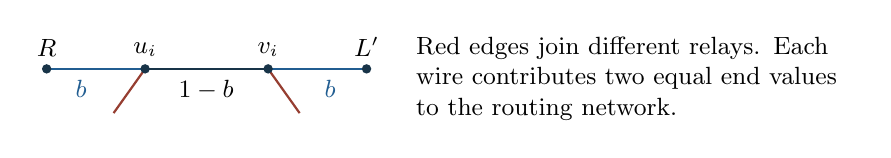
\begin{tikzpicture}[x=1.25cm,y=.78cm,every node/.style={font=\small},thick]
\draw[blueink] (0,0)--(1,0);
\draw[ink] (1,0)--(2.25,0);
\draw[blueink] (2.25,0)--(3.25,0);
\draw[rust] (1,0)--(.68,-.72);
\draw[rust] (2.25,0)--(2.57,-.72);
\foreach \x/\lab in {0/R,1/u_i,2.25/v_i,3.25/L'}{
\fill[ink] (\x,0) circle(1.7pt); \node[above] at (\x,.03) {$\lab$};}
\node[below,blueink] at (.35,-.01) {$b$};
\node[below] at (1.62,-.01) {$1-b$};
\node[below,blueink] at (2.88,-.01) {$b$};
\node[anchor=west,align=left,text width=5.55cm,font=\small] at (3.65,-.16)
{Red edges join different relays. Each wire contributes two equal end values to the routing network.};
\end{tikzpicture}
\end{center}

\sh{Two disjoint blue probes.}
On each of the two distinct closure wires through \(h_0,h_1\), replace the middle edge \(u_iv_i\) by a path \(u_i,p_1,\ldots,p_8,v_i\). Add the chords
\[
                   (1,4),\ (3,6),\ (5,8),\ (7,2)
\]
between the indicated internal vertices. Pick \(j=3\) on the first wire and \(j=4\) on the second. Prescribe \(p_jp_{j+1}\) blue and prescribe red on the two chords avoiding its endpoints. With red endpoints removed, the other four vertices form a four-vertex path with a unique perfect matching on its two chords. Forbidding the blue edge splits that path into two isolated edges. Thus all four chords are red in every candidate. Alternation along the long path forces blue on the first wire value and green on the second. Every prescribed edge in the entire graph is disjoint from every other.

\begin{center}
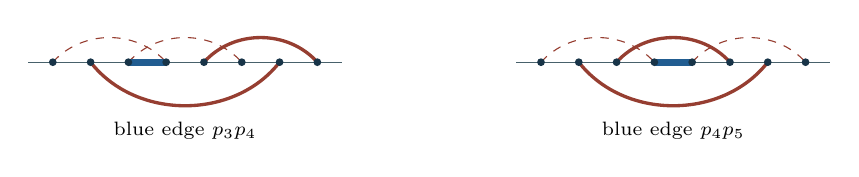
\begin{tikzpicture}[x=.48cm,y=.6cm, every node/.style={font=\scriptsize}]
\foreach \shift/\j in {0/3,6.2/4}{
\begin{scope}[xshift=\shift cm]
\draw[muted] (.35,0)--(8.65,0);
\foreach \a/\b in {1/4,3/6,5/8,2/7}{
 \pgfmathtruncatemacro{\p}{(\a==\j)||(\a==\j+1)||(\b==\j)||(\b==\j+1)}
 \ifnum\a=2\def\angle{52}\else\def\angle{-48}\fi
 \ifnum\p=1 \draw[rust,dashed] (\a,0) to[bend right=\angle] (\b,0);
 \else\draw[rust,line width=1.2pt] (\a,0) to[bend right=\angle] (\b,0);\fi}
\draw[blueink,line width=2.6pt] (\j,0)--({\j+1},0);
\foreach \i in {1,...,8}{\fill[ink] (\i,0) circle(1.4pt);}
\node at (4.5,-1.45) {blue edge \(p_{\j}p_{\the\numexpr\j+1\relax}\)};
\end{scope}}
\end{tikzpicture}
\end{center}

\sh{Graph checks.}
Put \(L,u_i,p_{\rm even}\) on one side and \(R,v_i,p_{\rm odd}\) on the other. All edges cross. Chords and path edges are distinct. Relay vertices are unique to their wires, so self-feedback at the logical level creates no loops or parallel graph edges. Before inserting the probes, the middle relay edges and red relay edges form a single cycle visiting all relays. The substituted paths preserve connectivity, and all switch vertices attach to relays. Every vertex has degree three. There are \(2w\) switch vertices, \(2w\) original relay vertices and \(16\) probe vertices. Exactly \(w+4=N/4\) edges are prescribed red.

\newpage
\Sec{The threshold, number of extensions and marginals}
\sh{Every matching corresponds to one assignment.}
The red relay edges, the four pinned probe chords and the four forced probe chords exhaust the red choices outside the variable cycles. On each variable cycle a red matching takes exactly one alternating half. Hence there are \(2^n\) red matchings, all avoiding both probes. Each matching gives \(n\) internal residual cycles and \(W-m\) program cycles. Set \(h=n+W-m\).

Under \(M_x\) the two probes lie on separate program cycles if \(F(x)=1\), and on the same program cycle if \(F(x)=0\). The first probe demands one wire value and the second demands its opposite. In the former case two cycles have their orientations fixed and the other \(h-2\) can alternate freely. In the latter case exactly one cycle is inconsistent. This proves both \(B(M_x)=1-F(x)\) and
\[
   \#\{\text{extendible red matchings}\}=\cnt(F),\qquad
   \#\{\text{labeled full extensions}\}=2^{h-2}\cnt(F).
\]
The number of extendible red matchings belongs to \(\#\mathrm P\) because a guessed matching can be checked in polynomial time by testing its residual cycles. Its hardness reduction is parsimonious. Counting full extensions is \(\#\mathrm P\)-complete under a polynomial-time metric reduction that divides by the displayed factor. A full coloring certifies membership of the decision problem in NP.

\sh{Why a single blue clue is easier.}
In any cubic bipartite graph, test for a red perfect matching containing all red clues and avoiding the single blue edge, if present. Reject conflicting forced red edges. Delete their endpoints, omit the forbidden edge and run bipartite matching on the remaining vertices. If this succeeds, every residual cycle is even and can be alternated. At most one cycle has an orientation prescribed. This proves sufficiency and gives a full coloring. It also proves the polynomial side for arbitrary placements of red clues.

\sh{Two-edge probability with an easy background count.}
Release both blue probes but retain every red clue. There are \(2^{n+h}\) labeled full colorings. Select each matching half by a fair coin and independently select the orientation of each of its \(h\) cycles. This samples exactly uniformly in linear time. Under this distribution each probe is blue with probability \(1/2\), since each is always nonred. For their joint event,
\[
               \Pr[\text{both blue}\mid\text{red clues}]
                         =\frac{\cnt(F)}{4\cdot2^n}.
\]
Computing this probability exactly is \(\#\mathrm P\)-hard, and deciding whether it is positive is NP-complete. An efficient sampler can miss an event of probability \(1/(4\cdot 2^n)\) on a uniquely satisfiable formula.

\sh{A worked instance.}
For \((x\lor y)(\neg x\lor y)(x\lor\neg y)\), with juxtaposition meaning conjunction, the graph has 1,560 vertices. Four red matchings encode \(00,01,10,11\). Their scores are \(1,1,1,0\). Only \(11\) extends and it gives \(2^{21}=2{,}097{,}152\) full colorings. The four probabilities for blue/blue, blue/green, green/blue, green/green are \(1/16,7/16,7/16,1/16\), respectively.

\newpage
\Sec{Exact algorithms and lower bounds}
\sh{The independent cycle parameter.}
Given a graph with these two clue colors, delete the endpoints of forced red edges and omit blue edges from the remaining red-matching graph \(H\). Reject conflicting forced edges. Suppose \(\Delta(H)\le2\). Each component is an isolated vertex, path or even cycle. A component with an odd number of vertices precludes a red perfect matching. Every even-order path has one possible matching. Each of the \(c\) cycles has two. Enumerate the \(2^c\) choices and scan the complement of each red matching in the original graph. This decides extension and counts all colorings in \(O^*(2^c)\) time and polynomial space. \(O^*\) suppresses polynomial factors, including integer arithmetic for counts.

\sh{Strong Exponential Time Hypothesis.}
For every fixed \(\epsilon>0\), an \(O^*((2-\epsilon)^c)\) decision algorithm on this class would refute SETH. On the constructed graph \(H\) is exactly \(n\) independent cycles and four isolated edges. Thus \(c=n\), independently of the formula width. Applying the hypothesized algorithm to \(k\)-CNF gives \(O^*((2-\epsilon)^n)\) for \emph{every} fixed \(k\), contrary to SETH \cite{ip}. This is a conditional lower bound for a structural parameter. NP-completeness itself is unconditional.

\sh{Ordinary exponential time and bounded cycle lengths.}
For 3-CNF the graph size is \(O(n+m)\), so \(2^{o(N)}\) time on the hard family would refute ETH by sparsification \cite{ipz}. Decision hardness persists if every free cycle has length at most 514. Replace a variable with \(d>1\) occurrences by distinct copies, one per occurrence, and add the \(d\) implications from each copy to the next cyclically. A true copy forces every copy true. Otherwise every copy is false. Padding each binary implication by repeating its consequent creates no variable of occurrence greater than four. Variables with one occurrence need no implication. Starting from ordinary 3-CNF gives a linear enlargement and \(128\cdot4+2=514\). The copy construction preserves model counts. The preceding SETH statement uses the original \(c=n\) reduction.

\sh{Distance between clues.}
For any prescribed constant distance, the exactly-two-blue decision problem stays NP-complete even with all clues that far apart. Replace each prescribed edge by a chain of \(2t\) copies of the graph of a cube with one edge removed and pin the central connector to its old color. Each copy has just two terminal edges. For each color, a perfect matching crosses the eight-vertex cut an even number of times. The two terminal colors must agree. Any common color extends by a coordinate coloring of the cube. The poles are at distance three, and two new clues have endpoint distance at least \(8t\). The graph stays simple, connected and cubic bipartite. Taking \(t\) to be a sufficiently large fixed power of the original order gives, for every fixed \(0<\delta<1\), \(O(N'^\delta)\) clues and separation \(\Omega(N'^{1-\delta})\) at output order \(N'\). The cycle parameter was measured before this spacing operation.

\newpage
\Sec{What a local move can reach}
\sh{Matchings that still extend.}
Allow one move to replace a red perfect matching by its symmetric difference with one alternating cycle, requiring the new matching to admit some full extension. On our graphs the symmetric difference between any two candidate matchings consists precisely of the variable cycles whose bits differ. Hence the graph of extendible red matchings with these moves is \emph{isomorphic} to the solution graph of \(F\) under single-variable flips.

It follows that deciding reachability between two given extendible red matchings is PSPACE-complete. Gopalan and coauthors prove the corresponding reachability theorem for 3-CNF \cite{gkmp}. Produce the two endpoint matchings by taking the indicated alternating halves. In the reverse complexity bound, store the current matching, guess its successor, check the symmetric difference and test the residual cycles. A counter with \(O(|E|)\) bits suffices for a simple path among at most \(2^{|E|}\) matchings. Nondeterministic polynomial space equals PSPACE.

\sh{Full colorings with fixed clues.}
A Kempe move interchanges two colors on one connected component of their two-color subgraph while preserving every clue. Here each such component is an even cycle. This move keeps the current full coloring as part of the state.

Append the tautology \((x_i\lor\neg x_i)\) for each variable \(i\) before compiling. It preserves every assignment. On a satisfying assignment, the central layer-zero path arrives at each clause in its initial central group and returns there after that clause. In the added tautology its first guard touches the module for \(i\) on \emph{both} rails, whatever the guard's truth value. During that forward pass each marked orbit therefore uses an internal nonred edge of the \(i\)-cycle. The two marked wire values are opposite, so those two internal edges have opposite colors in every full lift.

Every red-changing Kempe move would reach a different red matching. The changed edges form a single cycle, which must be one variable cycle. But its nonred edges include both blue and green. Consequently that cycle cannot be swapped with red in any full lift. Within a fixed red matching, each of the \(h-2\) unpinned blue-green cycles can be flipped independently. Each satisfying assignment gives exactly one Kempe component, itself a hypercube of dimension \(h-2\).

\note{\textbf{Counting components.} In the tautology-augmented graphs the number of clue-preserving Kempe classes equals \(\cnt(F)\) exactly. Thus counting classes is \(\#\mathrm P\)-hard. For two given colorings in this family, class membership is decidable by comparing their red matchings.}

\sh{Connectedness with a supplied solution.}
For a source formula \(F\), use a selector \(y\), clauses \(y\lor\neg x_i\) for each variable, and \(\neg y\lor C\) for each source clause \(C\). There is one solution with \(y=0\) and \(\cnt(F)\) with \(y=1\). Apply the tautology augmentation. A coloring for the known \(y=0\) assignment is constructible in polynomial time. The full Kempe graph is connected exactly when \(F\) is unsatisfiable, proving coNP-hardness even when an initial coloring is supplied.

\newpage
\Sec{Two restrictions that change the analysis}
\sh{Square switches.}
Consider the directed relay network of Section 3 when each internal switch has exactly two inputs and two outputs. Its square permits both possible bijections. Give any set of wires required binary values, using their physical parity to interpret the clues. A solution exists exactly when the wires assigned value one can form an integral circulation with unit capacities and the prescribed lower and upper bounds fixed to the requested bit. At each switch conservation equates the numbers of one-valued inputs and outputs. A bijection can then match ones to ones and zeros to zeros. Integral circulation with integer bounds has a polynomial-time decision and construction algorithm.

For just two opposite prescribed values, let \(a\) be the required one-arc and \(b\) the required zero-arc. A single directed cycle through \(a\) avoiding \(b\) suffices. Conversely a feasible integral circulation decomposes into directed cycles, one of which contains \(a\). Reachability from the head of \(a\) to its tail after deleting \(a,b\) therefore decides this case in linear time, with a loop treated as a cycle of length one. This concerns the coherent directed wire construction. Larger cyclic switches in the general reduction synchronize several visits to one Boolean variable.

\sh{A planar crossing obstruction.}
Place a gadget inside a disk. Its four boundary terminals, in cyclic order \(1,2,3,4\), must carry nonred colors. Internal clues may prescribe red only, and every internal vertex is cubic. No such planar bipartite gadget can transmit two independent binary wires across each other, with terminal equalities \(1=3\) and \(2=4\).

\begin{center}
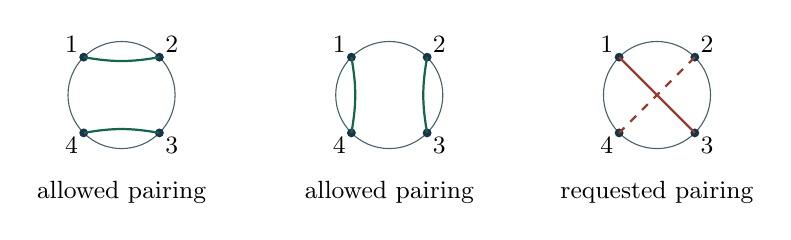
\begin{tikzpicture}[x=1cm,y=1cm,every node/.style={font=\small},thick]
\foreach \x/\name in {0/{allowed pairing},3.4/{allowed pairing},6.8/{requested pairing}}{
 \draw[muted,thin] (\x,0) circle (.68);
 \foreach \a/\n in {135/1,45/2,-45/3,-135/4}{
  \fill[ink] (\x,0) ++(\a:.68) circle(1.6pt);
  \node at ($(\x,0)+(\a:.90)$) {\n};}
 \node[below] at (\x,-.96) {\name};}
\draw[accent] (135:.68) to[bend right=10] (45:.68);
\draw[accent] (-135:.68) to[bend left=10] (-45:.68);
\begin{scope}[xshift=3.4cm]
\draw[accent] (135:.68) to[bend left=10] (-135:.68);
\draw[accent] (45:.68) to[bend right=10] (-45:.68);\end{scope}
\begin{scope}[xshift=6.8cm]
\draw[rust] (135:.68)--(-45:.68);
\draw[rust,dashed] (45:.68)--(-135:.68);\end{scope}
\end{tikzpicture}
\end{center}

Fix any feasible red matching on the interior. Its complement consists of internal even cycles and two disjoint paths pairing the terminals. Planarity forces a noncrossing pairing. Each path admits two alternating orientations independently, fixing an equality or an inequality between its endpoints. This gives four boundary strings. To realize the four requested strings exactly, every feasible matching would have to give those same four strings. For either noncrossing pairing, its path constraint relates one endpoint of each of the two independent crossing wires, and fails on some requested string. Taking a union of the four-string sets cannot repair this. The argument also excludes signed crossovers after relabeling the two values at individual terminals.

The complexity of the planar two-blue case and the case of two clues of each color remain undetermined by this construction. On a planar graph one can condition on all edge colors incident to a balanced \(O(\sqrt{N})\)-vertex separator and recurse \cite{lt}. The geometric sum along a recursion path is \(O(\sqrt N)\), giving \(2^{O(\sqrt N)}N^{O(1)}\) time for planar cubic inputs. Under ETH a reduction from sparse 3-SAT on \(n\) variables to this planar class cannot always output \(o(n^2)\) vertices.

\newpage
\Sec{Reproducibility and comparison with prior work}
\begingroup\small
\sh{Raw graph tests.}
The companion archive contains the DIMACS compiler, a red-matching enumerator, an independent all-different backtracker, and an optional Z3 check. Each graph edge carries its endpoints and one clue value. The enumerator reconstructs components from the raw graph. Decoder edge indices are used only to compare already generated matchings with variable assignments. The generic backtracker and Z3 use only vertex incidence and precolors.

\begin{center}\small
\begin{tabular}{@{}p{.33\linewidth}p{.60\linewidth}@{}}\toprule
Check & Observed outcome\\\midrule
Exhaustive assignment comparison & 404 compiled formulas, 3,266 assignments, 1,669 true and 1,597 false. Every conflict score, cycle count and lift multiplicity agreed. Every returned witness satisfied all edges.\\[3pt]
Exhaustive formula families & Included all 256 subsets of eight signed 3-clauses on three distinct variables and every signed length-three clause over two variables with repetition.\\[3pt]
Independent generic colorers & The backtracker counted 64, 64, 0 and 2,048 extensions for four one-variable instances. Z3 independently decided three SAT and three UNSAT instances up to 6,172 vertices, with no compiler metadata.\\[3pt]
Larger planted instance & 123,088 vertices and 48 variable cycles. The planted solution, all 48 single-bit changes and the all-zero assignment were checked. This run sampled 50 of \(2^{48}\) states.\\[3pt]
Kempe and marginals & 40 tautology-augmented graphs, 368 assignments. All 1,648 candidate red flips by color failed across the corresponding full fibers. Both one-edge marginals and the joint count matched the formulas.\\[3pt]
Sampler and controls & All 512 fair-coin tapes for the unit formula produced 512 distinct background colorings. Also checked 4,750 opposite-wire queries on 125 square networks and all eight signed noncrossing four-terminal patterns.\\\bottomrule
\end{tabular}
\end{center}

\sh{Prior art and scope.}
Kratochv\'il and Seb\H{o}'s perfect-graph vertex-precoloring theorem already gives hardness for two classes of size two on that broader graph class \cite{ks}. Fiala proved cubic bipartite edge-extension hardness \cite{fiala}. Fiala, Kratochv\'il and P\'or explicitly recorded the unrestricted two-preassigned-color version \cite{fkp}. Casselgren noted that Fiala's reduction itself uses two colors \cite{cass}. Bang-Jensen and Casselgren gave a replacement gadget \cite{bc}. Marx proved hardness with planarity and unrestricted clue multiplicities \cite{marx}. These cubic bipartite statements allow unbounded numbers of clues in both colors.

Belcastro and Haas studied edge-Kempe classes of cubic graphs, including structural results for planar bipartite graphs without fixed clues \cite{bh}. A recent Boolean orientation dichotomy concerns fixed local constraint languages \cite{eo}. The extra requirements here are two named minority edges, one red choice per source variable, uniform lift counts, and a concrete individual-assignment correspondence. I found no source in this search stating that combined result. Establishing publication priority would require a broader bibliographic and expert review.

\sh{Replication.}
The archive README gives the commands for regenerating a graph, solving it, sampling and running all checks. The core scripts require Python 3.10 or later. The separate general-purpose SAT cross-check uses Z3.

\newpage
\endgroup
\phantomsection\pdfbookmark[1]{References}{references}
{\LARGE\bfseries\color{ink} References\par}
{\small Linked articles and author manuscripts.}\par
\begingroup\small
\renewcommand{\refname}{}
\vspace{-1.0em}
\begin{thebibliography}{12}\setlength{\itemsep}{4.5pt}\setlength{\parskip}{0pt}
\bibitem{ks} J. Kratochv\'il and A. Seb\H{o}. \rref{https://pagesperso.g-scop.grenoble-inp.fr/~seboa/sebo_files/papers/jgt97prext.pdf}{Coloring precolored perfect graphs}. \emph{Journal of Graph Theory} 25 (1997), 207--215. Theorem 2.3 concerns the perfect-graph vertex problem.
\bibitem{fiala} J. Fiala. \rref{https://doi.org/10.1002/jgt.10088}{NP completeness of the edge precoloring extension problem on bipartite graphs}. \emph{Journal of Graph Theory} 43 (2003), 156--160. See also the \rref{https://kam.mff.cuni.cz/~fiala/papers/dis.pdf}{author's thesis}, Section 3.1.2.
\bibitem{fkp} J. Fiala, J. Kratochv\'il and A. P\'or. \rref{https://doi.org/10.1016/j.endm.2005.05.012}{On the computational complexity of partial covers of Theta graphs}. \emph{Electronic Notes in Discrete Mathematics} 19 (2005), 79--85, especially p.~81.
\bibitem{cass} C. J. Casselgren. \rref{https://doi.org/10.1016/j.disc.2011.10.028}{On avoiding some families of arrays}. \emph{Discrete Mathematics} 312 (2012), 963--972. Section 3, Problems 1 and 2.
\bibitem{bc} J. Bang-Jensen and C. J. Casselgren. \rref{https://doi.org/10.1016/j.dam.2015.04.020}{Restricted cycle factors and arc-decompositions of digraphs}. \emph{Discrete Applied Mathematics} 193 (2015), 80--93. Problem 2.3.
\bibitem{marx} D. Marx. \rref{https://www.cs.bme.hu/~dmarx/papers/planar-edge-prext.pdf}{NP-completeness of list coloring and precoloring extension on the edges of planar graphs}. \emph{Journal of Graph Theory} 49 (2005), 313--324. Theorem 2.3.
\bibitem{ip} R. Impagliazzo and R. Paturi. \rref{https://doi.org/10.1006/jcss.2000.1727}{On the complexity of \(k\)-SAT}. \emph{Journal of Computer and System Sciences} 62 (2001), 367--375.
\bibitem{ipz} R. Impagliazzo, R. Paturi and F. Zane. \rref{https://cseweb.ucsd.edu/~paturi/myPapers/pubs/ImpagliazzoPaturiZane_2001_jcss.pdf}{Which problems have strongly exponential complexity?} \emph{Journal of Computer and System Sciences} 63 (2001), 512--530.
\bibitem{gkmp} P. Gopalan, P. G. Kolaitis, E. Maneva and C. H. Papadimitriou. \rref{https://doi.org/10.1137/07070440X}{The connectivity of Boolean satisfiability: computational and structural dichotomies}. \emph{SIAM Journal on Computing} 38 (2009), 2330--2355. Section 3.3.
\bibitem{bh} s.-m. belcastro and R. Haas. \rref{https://arxiv.org/abs/1209.1730}{Counting edge-Kempe-equivalence classes for 3-edge-colored cubic graphs}. \emph{Discrete Mathematics} 325 (2014), 77--84.
\bibitem{eo} J. Guan, S. Shao and K. Shi. \rref{https://keshi.pro/files/papers/eo-dichotomy.pdf}{A dichotomy for constrained Eulerian orientations}. Author manuscript, consulted 21 November 2026.
\bibitem{lt} R. J. Lipton and R. E. Tarjan. \rref{https://www.cs.princeton.edu/courses/archive/fall06/cos528/handouts/sepplanar.pdf}{A separator theorem for planar graphs}. \emph{SIAM Journal on Applied Mathematics} 36 (1979), 177--189.
\bibitem{clay} Clay Mathematics Institute. \rref{https://www.claymath.org/millennium/p-vs-np/}{P vs NP}. Official Millennium Problem status, consulted 21 November 2026.
\end{thebibliography}\endgroup
\end{document}
